\section{Box}

\subsection*{Design Overview}
\begin{table}[h!]
\centering
\begin{tabular}{l|p{0.62\textwidth}}
\toprule
\textbf{Parameter} & \textbf{Specification} \\ \bottomrule
Base Material & \textcolor{orange}{Aluminum 6061} or \textcolor{orange}{gold-plated copper} \footnotemark \\
pedestal drill $\Delta$ & \textcolor{orange}{3.8 mm in arXiv:1906.05425 (the chip on four corner posts). Here the floor under the die is recessed instead: a circle ($\varnothing$6.25 mm) or a rounded square (6.2 mm, corner radius 1 mm), 0.2 to 0.5 mm deep in the simulations. Shape and depth are under study.} \\
\bottomrule
\end{tabular}
\end{table}
\footnotetext{need to review alternatives. Per arXiv:1906.05425: aluminium superconducts (no conductor loss at millikelvin temperatures), but its thermal conductivity is limited and it forms an oxide; copper is a normal metal with high thermal conductivity and forms an oxide; gold-plated copper is a normal metal with high thermal conductivity and a limited oxide. The conductor loss of the paper's Fig.~2e concerns the normal-metal boxes.}

\subsection*{Design Checklist}

\begin{itemize}[label={$\square$}]
    \item mounting wings to connect to the refrigerator.
    \item Parasitic Control -- Minimize cavity modes and conductivity loss (\href{https://arxiv.org/abs/1906.05425}{arXiv:1906.05425}). Status of the simulations:
    \begin{itemize}[label={--}]
        \item With the die on a flat floor (the paper's solid pedestal) the chip has a mode at 6.843 GHz, in the 5--9 GHz band: S21 down to $-30$ dB, 18 MHz wide, almost total reflection. A recess under the die of 0.2 to 0.5 mm removes it.
        \item A box mode at 6.90 GHz remains whatever the floor. It is $-2.5$ dB deep and 1.7 MHz wide on RO3003 ($-18$ dB and 4.8 MHz on TMM10i). The next box mode of the eigenmode run (TMM10i, bare board) is at 9.28 GHz.
        \item \textcolor{red}{To do: the conductor loss against the gap under the die (the paper's Fig.~2e) for each pocket shape and depth, and the choice of shape and depth from it.}
    \end{itemize}
    \item Tightness (the box should close the PCB from all sides). The vents (air under the die and in the screw bores) are cut after the box is made; the simulations have none.
    \item Anchoring to the refrigerator.
\end{itemize}
\begin{figure}[h]
    \centering
    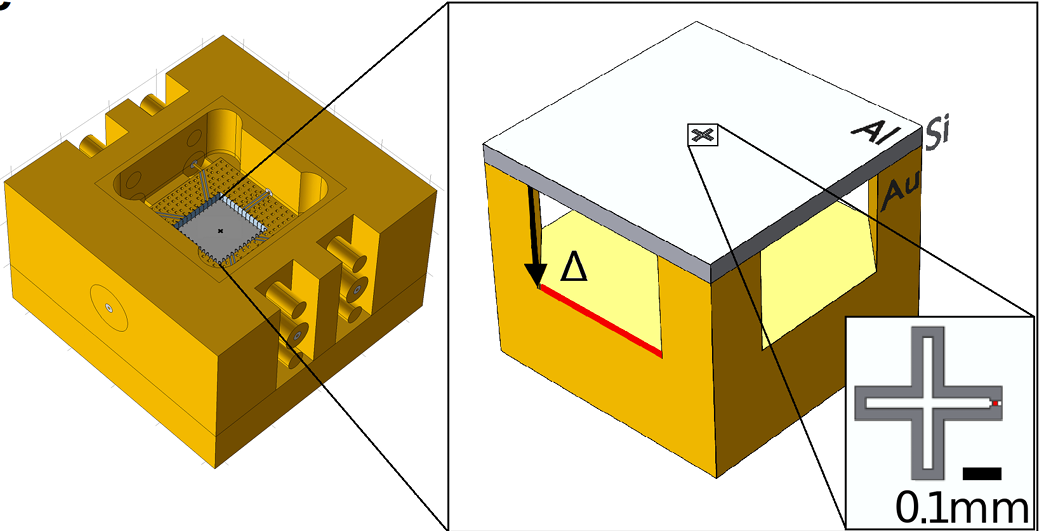
\includegraphics[width=0.6\linewidth]{tex/box example.png}
\end{figure}
